\begin{center}
    \begin{figure}[H]
        \centering

        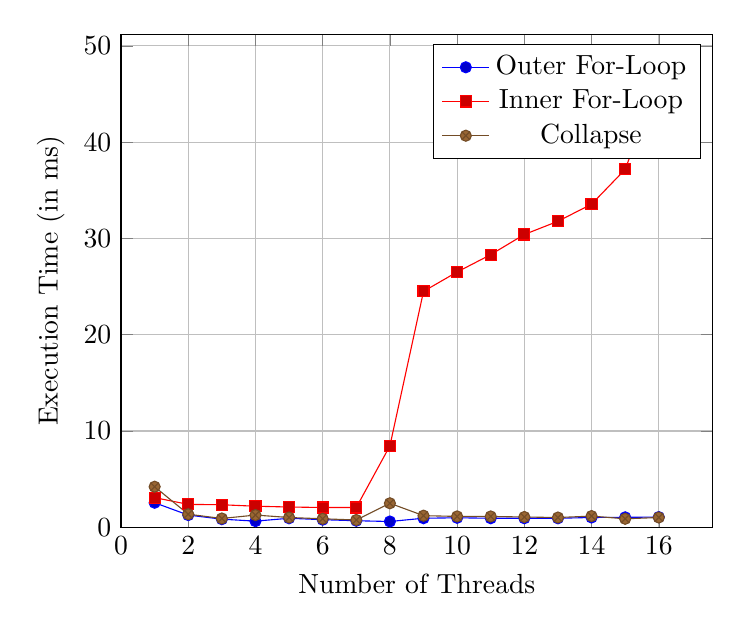
\begin{tikzpicture}
            \begin{axis}[
                title={},
                width=0.75\textwidth,
                xlabel={Number of Threads},
                ylabel={Execution Time (in ms)},
                xmin=0,
                ymin=0,
                grid=major
            ]
                \addplot coordinates {
                    (1,2.5549)(2,1.2735)(3,0.85025)(4,0.6436)(5,0.94375)(6,0.7966)(7,0.6854)(8,0.6077)(9,0.9472)(10,0.99225)(11,0.9471)(12,0.94635)(13,0.94125)(14,1.02495)(15,1.041)(16,1.06755)
                };
                \addlegendentry{Outer For-Loop}

                \addplot coordinates {
                    (1,3.08615)(2,2.3858)(3,2.34615)(4,2.19415)(5,2.1119)(6,2.0609)(7,2.06245)(8,8.4643)(9,24.5043)(10,26.5145)(11,28.3157)(12,30.4109)(13,31.7816)(14,33.5549)(15,37.1696)(16,46.544)
                };
                \addlegendentry{Inner For-Loop}       

                \addplot coordinates {
                    (1,4.2187)(2,1.36355)(3,0.92205)(4,1.27645)(5,1.0218)(6,0.8902)(7,0.76425)(8,2.5011)(9,1.21405)(10,1.13565)(11,1.1338)(12,1.0742)(13,1.0206)(14,1.17005)(15,0.88735)(16,1.0243)
                };
                \addlegendentry{Collapse}
            \end{axis}
        \end{tikzpicture}
        \caption{Grayscale Performance Tests dice.png}
    \end{figure}
\end{center}